\chapter{Thiết kế và thực hiện phần mềm}
\section{Thiết kế phần mềm cho thiết bị thu thập dữ liệu}
\subsection{Yêu cầu đặt ra cho phần mềm}
Thiết bị được thiết kế cho mục đích thu thập dữ liệu theo thời gian thực, yêu cầu có thể xử lý nhiều tác vụ 
song song với nhau, cụ thể hơn các yêu cầu thiết kế bao gồm:
\begin{itemize}
    \item \textbf{Tính ổn định khi hoạt động:} Yêu cầu quá trình thu thập dữ liệu từ các đồng hồ điện theo chu 
    kỳ, dữ liệu định kỳ được ghi vào bộ nhớ tại thiết bị và định kỳ gửi dữ liệu lên Cloud, có thể chuyển đổi qua
    phương thức kết nối mạng có dây khi kết nối mạng không dây không khả dụng.
    
    \item \textbf{Khả năng mở rộng và phát triển:} Cấu trúc chương trình cần hỗ trợ dễ dàng tích hợp thêm tính năng mới 
    hoặc thay đổi phần cứng mà không ảnh hưởng đến các chức năng hiện có trên thiết bị.

    \item \textbf{Dễ dàng cấu hình và cập nhật tính năng mới:} Cho phép nạp chương trình mới qua giao tiếp USB, trong quá trình
    phát triển thiết bị có thể in log ra console giúp thuận tiện trong việc phát hiện các lỗi tiềm ẩn, 
    giúp việc nâng cấp và bảo trì hệ thống trở nên thuận tiện.

    \item \textbf{Thiết kế giao diện người dùng:} Cho phép người dùng có thể tương tác với thiết bị với mục đích cấu hình
    một số các thông số cho thiết bị hoạt động.

    \item \textbf{Có khả năng lưu trữ dữ liệu:} Thiết bị sau khi thu thập dữ liệu sẽ được lưu trữ ngay trên thiết bị, phòng
    trường hợp thiết bị mất kết nối mạng vẫn có thể lưu trữ được dữ liệu theo thời gian. 
\end{itemize}

\subsection{Phương pháp thực hiện chương trình}
Để đáp ứng được yêu cầu quan trọng nhất là đáp ứng thời gian thực khi thu thập dữ liệu từ các đồng hồ điện, ngôn ngữ sử dụng 
chính trong quá trình viết phần mềm là C, với khả năng ngôn ngữ C có thể trực tiếp tác động lên phần cứng, kết hợp với sử dụng
hệ điều hành FreeRTOS, chính điều này giúp đáp ứng thời gian thực hơn các ngôn ngữ khác. 
Phương pháp triển khai chương trình
cụ thể cho từng yêu cầu ở trên như sau:
\begin{itemize}
    \item \textbf{Tính ổn định khi hoạt động:} Sử dụng FreeRTOS để chia hệ thống thành các Task độc lập (Task thu thập dữ liệu, 
    Task ghi Log, Task truyền tin), điều này giúp việc thu thập dữ liệu từ đồng hồ điện diễn ra đúng chu kỳ mà không bị ảnh 
    hưởng bởi việc truyền dữ liệu lên Cloud chậm. Phân tích logic kiểm tra trạng thái mạng. Hệ thống sẽ ưu tiên Wi-Fi, nếu mất 
    kết nối Wi-Fi sẽ tự động Chuyển qua gửi dữ liệu thông qua Ethernet để đảm bảo dữ liệu luôn được đẩy lên Cloud.
    
    \item \textbf{Khả năng mở rộng và phát triển:} Mỗi tính năng mới được xây dựng như một thư viện (Middleware) riêng biệt, 
    chỉ cần tích hợp vào hệ thống và tạo task dựa trên thư viện vừa tạo mà không can thiệp vào các Task cũ.

    \item \textbf{Dễ dàng cấu hình và cập nhật tính năng mới:} Sử dụng giao tiếp USB-to-UART, sử dụng thư viện in Log của ESP32  
    chuyển đổi để nạp chương trình và xuất Log ra terminal qua chuẩn UART của ESP32.  
    
    \item \textbf{Thiết kế giao diện người dùng:} Thiết kế ra các giao diện cố định hoặc giao diện động dựa trên chức năng đang
    thực hiện. Màn hình sẽ hiển thị các mục được định nghĩa trước để người dùng có thể lựa chọn thông qua các nút nhấn và encoder
    tích hợp sẵn trên thiết bị giao tiếp bằng GPIO. Về phần cấu hình Wi-Fi cho thiết bị có thể được thực hiện thông một Web Server 
    đơn giản, người dùng sẽ nhập SSID và Password bằng cách kết nối với Wi-Fi do ESP32 phát, giao diện nhập liệu Wi-Fi được viết 
    bằng ngôn ngữ HTML đơn giản và được lưu vào bộ nhớ Flash của ESP32.

    \item \textbf{Có khả năng lưu trữ dữ liệu:} Sử dụng thẻ nhớ SD Card được tích hợp thêm vào thiết bị và sử dụng giao thức SPI để
    ghi dữ liệu vào SD Card, chức năng ghi dữ liệu vào SD Card được tách thành một task riêng biệt chạy song song với các task khác 
    trong chương trình, điều này giúp cho khi thiết bị không có kết nối mạng, không thể gửi dữ liệu lên Cloud, thì dữ liệu vẫn được
    ghi vào thẻ nhớ. Người dùng có thể đọc được file ghi dữ liệu này dưới dạng file Excel, ứng với mỗi dữ liệu sẽ kèm theo mốc thời
    gian tại thời điểm ghi dữ liệu đó.
\end{itemize}

\subsection{Lưu đồ giải thuật chương trình}
\subsubsection{Kiến trúc tổng quát về tổ chức phần mềm}
\begin{figure}[H]
    \centering
    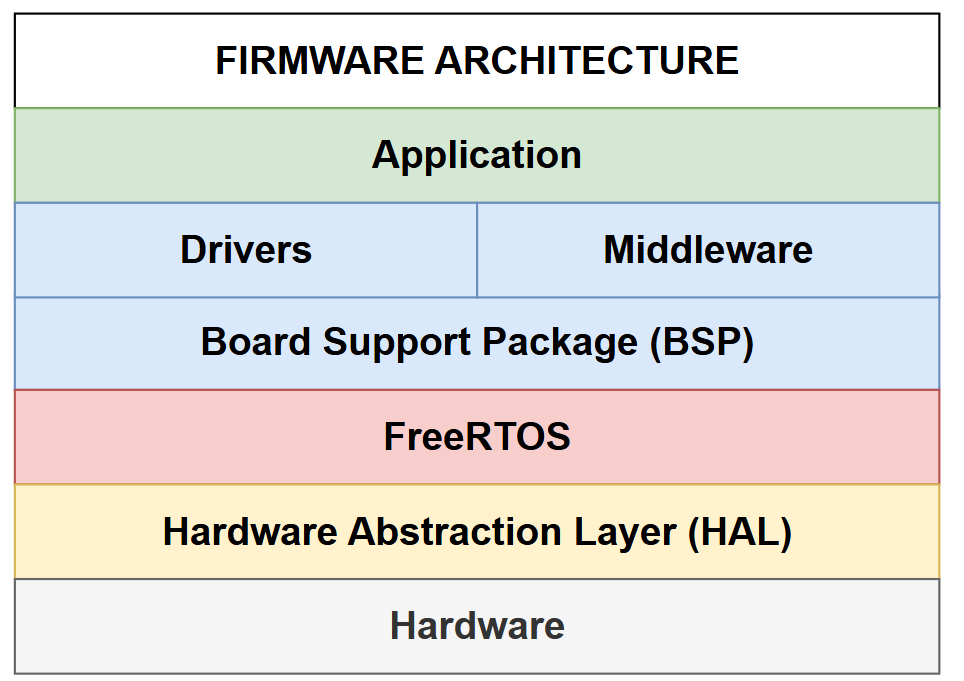
\includegraphics[width=0.6\textwidth]{image/tong_quat_firmware.png}
    \caption{Tổng quát kiến trúc phần mềm của thiết bị}
    \label{fig: tong_quat_firmware}
\end{figure}
\begin{itemize}
    \item \textbf{Application:} Lớp cao nhất, chứa logic thực hiện cốt lõi của hệ thống, nơi thực hiện các hoạt động theo yêu cầu của người dùng như
    thực hiện chu kỳ thu thập dữ liệu từ đồng hồ điện, Xử lý logic ghi dữ liệu vào bộ nhớ cục bộ khi mất mạng và đồng bộ hóa dữ liệu với Cloud khi có kết nối mạng,
    quản lý giao diện cấu hình thông số hệ thống và hiển thị trạng thái hoạt động của thiết bị, nơi định nghĩa các trang có thể hiển thị trên màn hình
    LCD.
    \item \textbf{Drivers và Middleware:} Drivers điều khiển các thiết bị ngoại vi cụ thể thông qua thư viện phần mềm, thực hiện viết phần mềm cấu hình,
    mô tả cách thức hoạt động cho các khối chức năng trên thiết bị. Middleware cung cấp các thư viện giao thức và dịch vụ thực hiện. Bao gồm các bộ thư 
    viện như Modbus Stack, stack TCP/IP trong LwIP của ESP32 cho Ethernet/Wi-Fi hoặc các thư viện mã hóa bảo mật khi gửi dữ liệu lên Cloud.

    \item \textbf{Board Support Package (BSP):} Tập hợp các định nghĩa phần cứng cụ thể cho thiết bị thông qua phần mềm, cấu hình các chân 
    kết nối và thiết lập môi trường hoạt động cho board mạch thực tế đang thiết kế, giúp kết nối giữa phần cứng và phần mềm.

    \item \textbf{FreeRTOS:} Đây là lớp nền tảng, chịu trách nhiệm quản lý đa nhiệm, cấp phát bộ nhớ, đồng bộ hóa tiến trình và quản 
    lý thời gian. FreeRTOS được tích hợp sẵn trong môi trường phát triển và được sử dụng xuyên suốt trong chương trình chính giúp điều phối
    hoạt động giữa các task đã khởi tạo

    \item \textbf{Hardware Abstraction Layer (HAL):} Lớp HAL giúp tách biệt phần mềm với phần cứng cụ thể, cung cấp các giao diện 
    trừu tượng để truy xuất phần cứng, được tích hợp sẵn trong bộ thư viện kèm theo khi sử dụng thư viện IDF của expressif. Cho phép phần mềm 
    tương tác với phần cứng (như đọc/ghi GPIO, cấu hình bộ định thời) mà không cần can thiệp trực tiếp vào địa chỉ bộ nhớ của chip. 
    Điều này giúp mã nguồn dễ dàng chuyển đổi sang các dòng chip khác trong tương lai nếu cần.

    \item \textbf{Hardware:} Bao gồm các tài nguyên phần cứng như vi điều khiển, bộ nhớ và các ngoại vi
    tích hợp, là cơ sở cho các tầng phần mềm phía trên hoạt động.Bao gồm vi điều khiển chính (ESP32-S3), các module tích hợp trên thiết bị  
    (W5500 cho Ethernet), các ngoại vi lưu trữ (thẻ nhớ SD), và các IC hỗ trợ đọc dữ liệu từ đồng hồ điện kết nối qua RS485. Thực hiện các 
    thao tác điện lý như đóng cắt tín hiệu, lưu trữ vật lý và truyền nhận dữ liệu thô qua các chân GPIO, UART, SPI.
\end{itemize}
\subsubsection{Lưu đồ giải thuật tổng quát}
\begin{figure}[H]
    \centering
    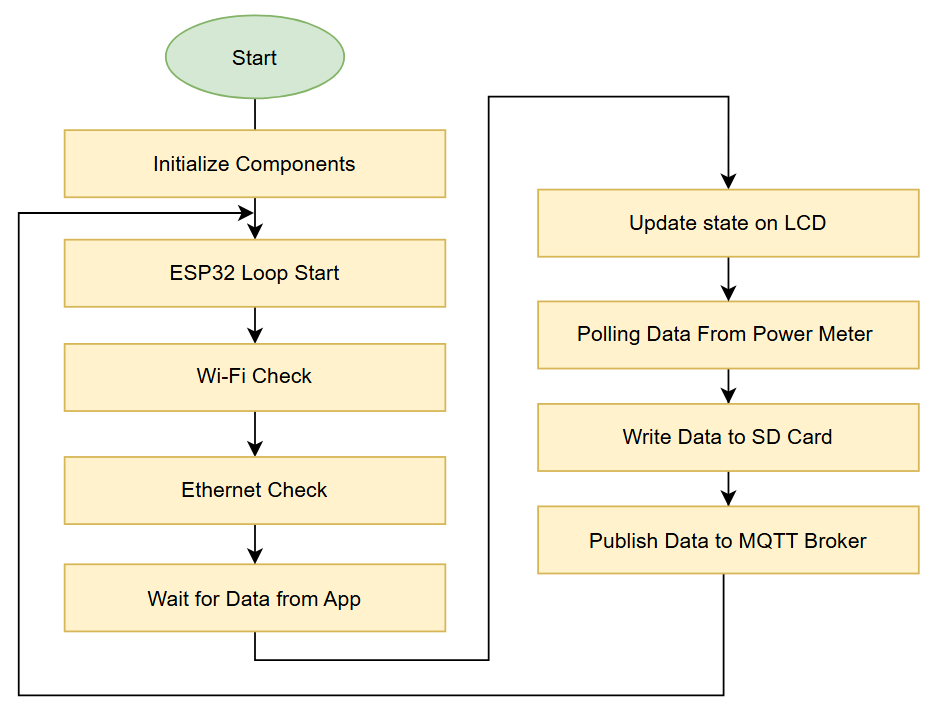
\includegraphics[width=0.8\textwidth]{image/flowchart_tong_quat_1.png}
    \caption{Lưu đồ giải thuật thực hiện tổng quát của hệ thống}
    \label{fig: flowchart_tong_quat_1}
\end{figure}
Lưu đồ này mô tả một cách tổng quát các hành vi có trong hệ thống, bao gồm:
\begin{itemize}
    \item \textbf{Start:} khởi đầu của chương trình ngay khi thiết bị được cấp nguồn hoặc khởi động lại (Reset).
    \item \textbf{Initialize Components:} Gọi các hàm khởi tạo của từng thành phần có trong thiết bị, gồm: Wi-Fi, Ethernet, Modbus RTU, Modbus TCP, SD Card, MQTT, User Interface
    \item \textbf{ESP32 Loop Start:} vòng lặp tuần hoàn, đảm bảo các tác vụ kiểm tra mạng, thu thập và gửi dữ liệu được thực hiện lặp đi lặp lại theo đúng trình tự.
    \item \textbf{Wi-Fi Check:}: Luôn kiểm tra tình trạng kết nối Wi-Fi trong quá trình thiết bị hoạt động, có thể chuyển đổi qua Ethernet khi mất mạng.
    \item \textbf{Ethernet Check:}: Luôn kiểm tra tình trạng kết nối Ethernet có dây trong quá trình thiết bị hoạt động, khi Wi-Fi có thể chuyển đổi qua sử dụng Ethernet.
    \item \textbf{Wait for Data from App:} Nhận gói tin chứa các thanh ghi cấu hình của các đồng hồ điện mới thêm vào hệ thống, hoặc xóa khỏi hệ thống. Các thanh ghi này 
    sẽ được phục vụ cho việc thu thập dữ liệu của thiết bị.
    \item \textbf{Polling Data Power Meter:} Chức năng chính của thiết bị, thu thập dữ liệu định kỳ các đồng hồ điện. Sử dụng giao thức Modbus RTU để gửi lệnh truy vấn (Request)
    đến các đồng hồ điện và nhận về (Response) các thông số định lượng như điện áp, dòng điện, công suất và điện năng tiêu thụ.
    \item \textbf{Write Data to SD Card:} Lưu trữ dữ liệu cục bộ ngay tại thiết bị. Dữ liệu vừa thu thập được sẽ được ghi vào thẻ nhớ SD. Việc này đảm bảo tính an toàn dữ liệu, 
    giúp lưu trữ thông tin theo thời gian thực ngay cả khi hệ thống mất kết nối mạng.
    \item \textbf{Publish Data to MQTT Broker:} Truyền tải thông tin đã xử lý lên máy chủ quản lý trung tâm. Đóng gói dữ liệu và gửi lên Cloud theo các giao thức truyền thông mạng. 
\end{itemize}

\subsection{Lưu đồ giải thuật chi tiết}
\begin{figure}[H]
    \centering
    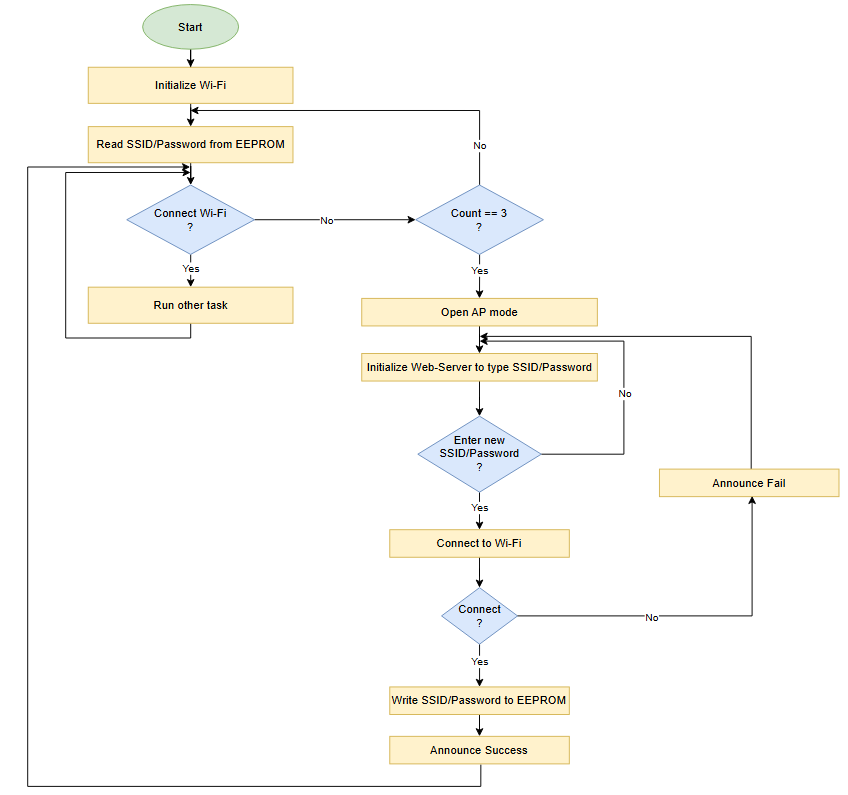
\includegraphics[width=0.9\textwidth]{image/wifi_config.png}
    \caption{Lưu đồ giải thuật cấu hình Wi-Fi}
    \label{fig: wifi_config}
\end{figure}
\begin{itemize}
    \item \textbf{Initialize Wi-Fi:} Khởi tạo trình các biến cấu hình cho Wi-Fi
    \item \textbf{Read SSID/Password from EEPROM:} Đọc thông tin mạng: tên Wi-Fi và mật khẩu đã lưu từ bộ nhớ EEPROM.
    \item \textbf{Connect Wi-Fi?:} Kiểm tra xem có kết nối thành công với thông tin đã đọc hay không.\\
    \textbf{Yes:}Chuyển sang thực hiện các tác vụ chính khác\\
    \textbf{No:} Kiểm tra số lần thử kết nối (Count == 3 ?). Nếu chưa đủ 3 lần, hệ thống sẽ quay lại thử lại.
    \item \textbf{Open AP mode:} Nếu thử lại 3 lần thất bại, thiết bị sẽ tự phát một mạng Wi-Fi riêng (Access Point) để người dùng kết nối vào.
    \item \textbf{Initialize Web-Server:} Khởi tạo một trang web nội bộ để người dùng có thể nhập tên Wi-Fi và mật khẩu mới.
    \item \textbf{Enter new SSID/Password ?:} Đợi người dùng nhập và gửi thông tin mạng mới từ trình duyệt.
    \item \textbf{Connect to Wi-Fi:} Thiết bị dùng thông tin mới vừa nhận được để thử kết nối lại.\\
    \textbf{Yes - Write SSID/Password to EEPROM:} Lưu thông tin mạng mới vào bộ nhớ để sử dụng cho những lần khởi động sau.\\
    \textbf{No - Announce Success:} Thông báo kết nối thành công và quay lại quy trình vận hành bình thường.
\end{itemize}

\begin{figure}[H]
    \centering
    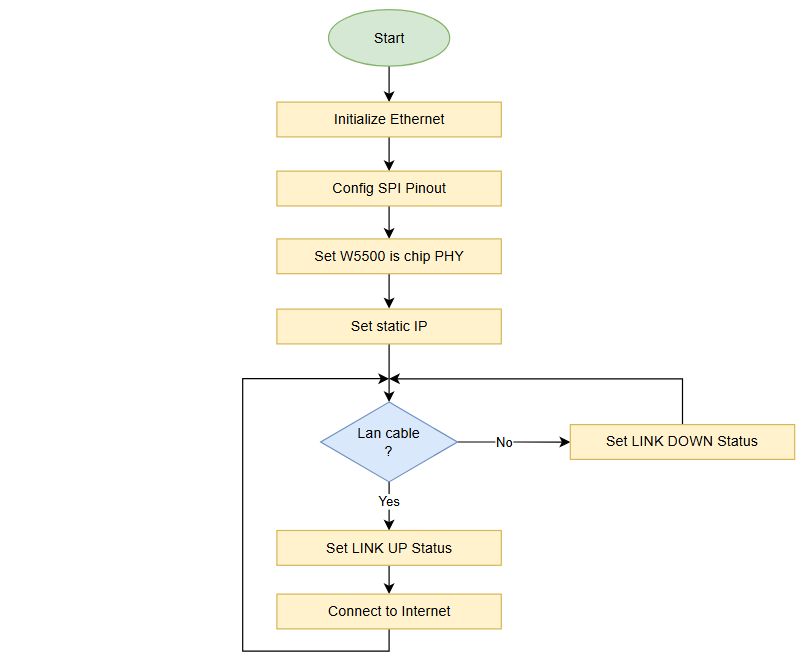
\includegraphics[width=0.8\textwidth]{image/eth_task.png}
    \caption{Lưu đồ giải thuật cấu hình Ethernet}
    \label{fig: eth_task}
\end{figure}
\begin{itemize}
    \item \textbf{Initialize Ethernet:} Bắt đầu quá trình khởi tạo các biến liên quan cho kết nối Ethernet.
    \item \textbf{Config SPI Pinout:} Cấu hình các chân tín hiệu của giao thức SPI: MOSI, MISO, SCK, CS để ESP32 có thể giao tiếp với chip W5500.
    \item \textbf{Set W5500 is chip PHY:} Chỉ định chip W5500 đóng vai trò là bộ điều khiển lớp vật lý PHY để xử lý tín hiệu mạng dây, sử dụng W5500 với chế độ MACRAW trong ESP32.
    \item \textbf{Set static IP:} Thiết lập địa chỉ IP tĩnh cố định cho thiết bị.
    \item \textbf{Lan cable ?:} Kiểm tra xem dây mạng LAN đã được cắm vào cổng RJ45 hay chưa.\\
    \textbf{No - Set LINK DOWN Status:} Nếu chưa có cáp, hệ thống xác lập trạng thái mất kết nối và tiếp tục vòng lặp kiểm tra.\\
    \textbf{Yes - Set LINK UP Status:} Nếu dây mạng đã cắm, thì xác nhận trạng thái kết nối vật lý thành công.
    \item \textbf{Connect to Internet:} Thiết bị thực hiện các giao thức mạng để kết nối ra Internet thông qua đường truyền Ethernet đã thiết lập.
\end{itemize}

\begin{figure}[H]
    \centering
    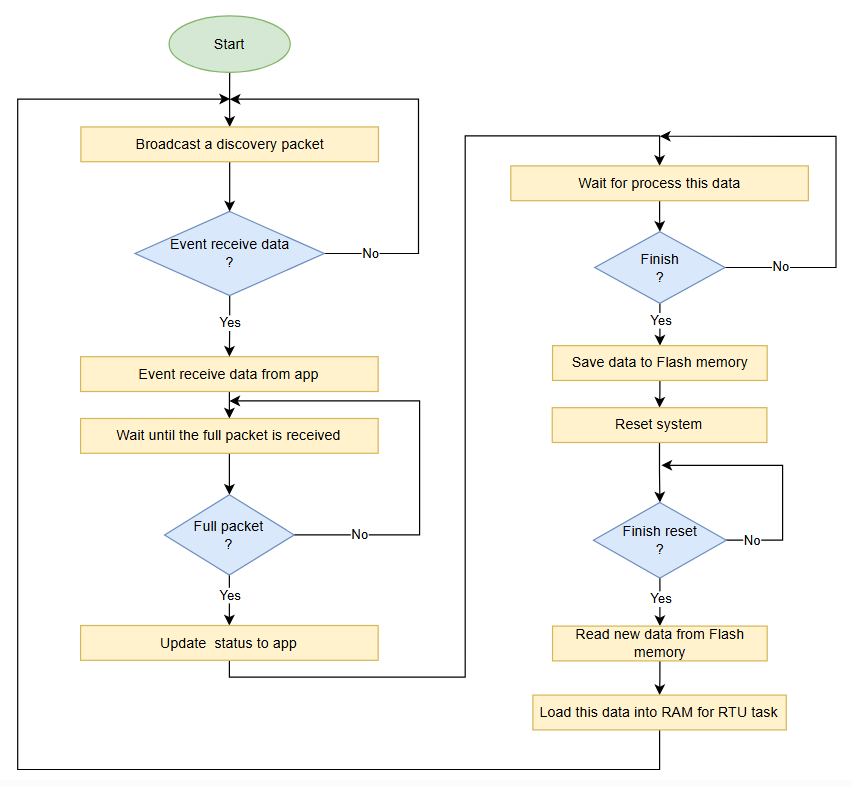
\includegraphics[width=0.85\textwidth]{image/receive_app.png}
    \caption{Lưu đồ giải thuật đợi nhận data từ App qua BLE}
    \label{fig: receive_app}
\end{figure}
\begin{itemize}
    \item \textbf{Broadcast a discovery packet:} Thiết bị phát các gói tin quảng bá ra không gian mạng để thông báo sự hiện diện của mình.
    \item \textbf {Event receive data ?:} Hệ thống kiểm tra xem có bất kỳ phản hồi hoặc dữ liệu nào gửi tới sau khi phát quảng bá không.\\
    \textbf {No:} Quay lại tiếp tục chờ kết nối từ App.\\
    \textbf {Yes:} Ghi nhận sự kiện nhận dữ liệu từ App.
    \item \textbf{Wait until the full packet is received:} chờ để đảm bảo nhận đầy đủ tất cả các phần của gói tin từ App gửi tới.
    \item \textbf{Full packet ?:} Kiểm tra xem toàn bộ nội dung gói tin đã được nhận đủ chưa, dựa vào kiểm tra dấu ngoặc vuông cuối cùng của gói tin JSON.\\
    \textbf {No:} Tiếp tục nhận và chờ.\\
    \textbf {Yes:} Gửi phản hồi thành công về App và bắt đầu xử lý lưu vào bộ nhớ Flash.
    \item \textbf{Wait for process this data:} Hệ thống tiến hành xử lý dữ liệu.
    \item \textbf{Finish?:} Xác nhận việc xử lý dữ liệu đã hoàn tất.
    \item \textbf{Save data to Flash memory:} Lưu các thông số mới vào bộ nhớ Flash.
    \item \textbf{Reset system:} Khởi động lại hệ thống.
    \item \textbf{Finish reset ?:} Đợi hệ thống hoàn tất quá trình tự kiểm tra sau khi khởi động lại.
    \item \textbf{Read new data from Flash memory:} Truy xuất các thông số vừa được lưu trước đó từ Flash.
    \item \textbf{Load this data into RAM for RTU task:} Nạp dữ liệu vào RAM để tác vụ Modbus RTU bắt đầu hoạt động với tập thanh ghi mới nhất.
\end{itemize}

\begin{figure}[H]
    \centering
    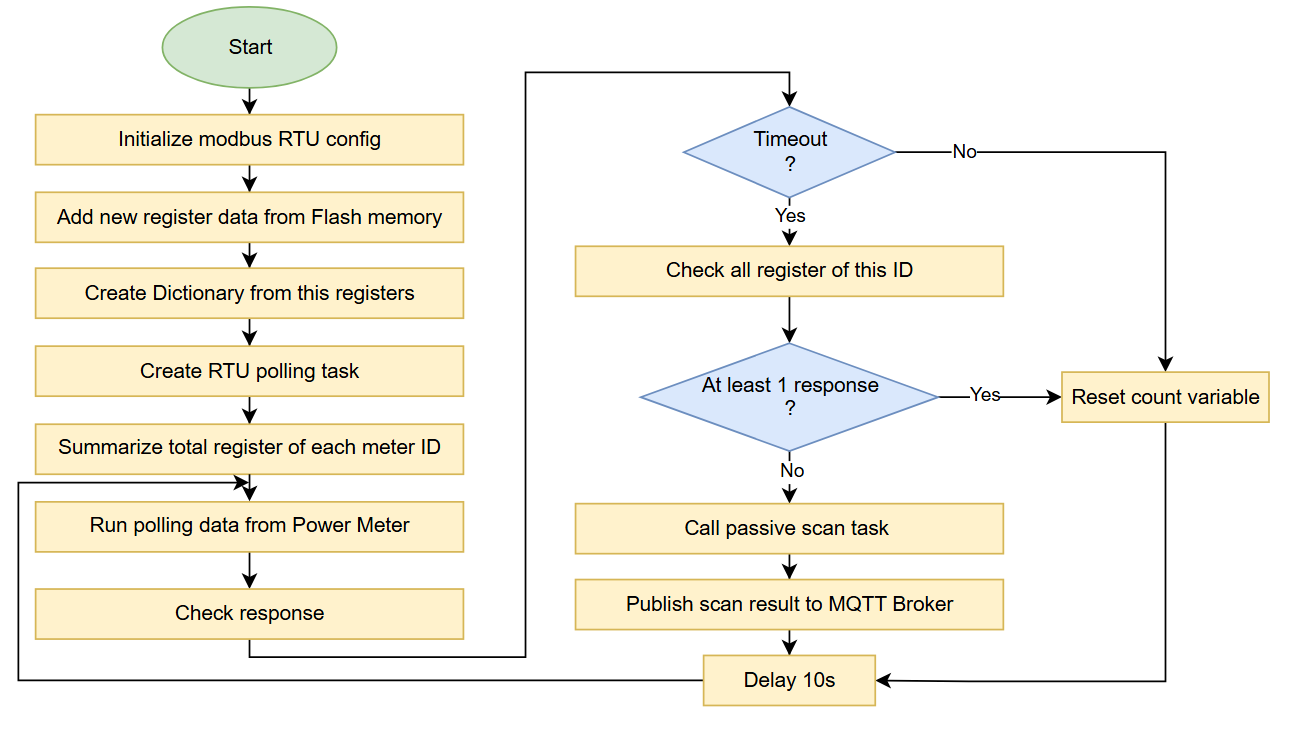
\includegraphics[width=0.5\textwidth]{image/rtu_task.png}
    \caption{Lưu đồ giải thuật thu thập dữ liệu từ đồng hồ điện}
    \label{fig: rtu_task}
\end{figure}
\begin{itemize}
    \item \textbf{Initialize modbus RTU config:} Thiết lập các thông số cấu hình cơ bản cho giao thức Modbus RTU (như cổng UART, parity, stop bits).
    \item \textbf{Add new register data from Flash memory:} Truy xuất danh sách tất cả các thanh ghi được lưu trữ sẵn trong bộ nhớ Flash đưa vào RAM.
    \item \textbf{Create Dictionary from this registers:} Tạo danh sách thanh ghi thành dạng "Dictionary" theo chuẩn chuẩn của thư viện esp-modbus dựa trên dữ liệu vừa được đưa vào RAM.
    \item \textbf{Create RTU polling task:} Tạo một task riêng cho việc thu thập dữ liệu từ các đồng hồ điện.
    \item \textbf{Run polling data from Power Meter:} Thực hiện việc gửi lệnh đọc và nhận dữ liệu thực tế từ đồng hồ đo điện thông qua đường truyền Modbus.
    \item \textbf{Delay 10s:} Cứ 10 giây thì chạy task thu thập dữ liệu đồng hồ điện một lần.
\end{itemize}

\begin{figure}[H]
    \centering
    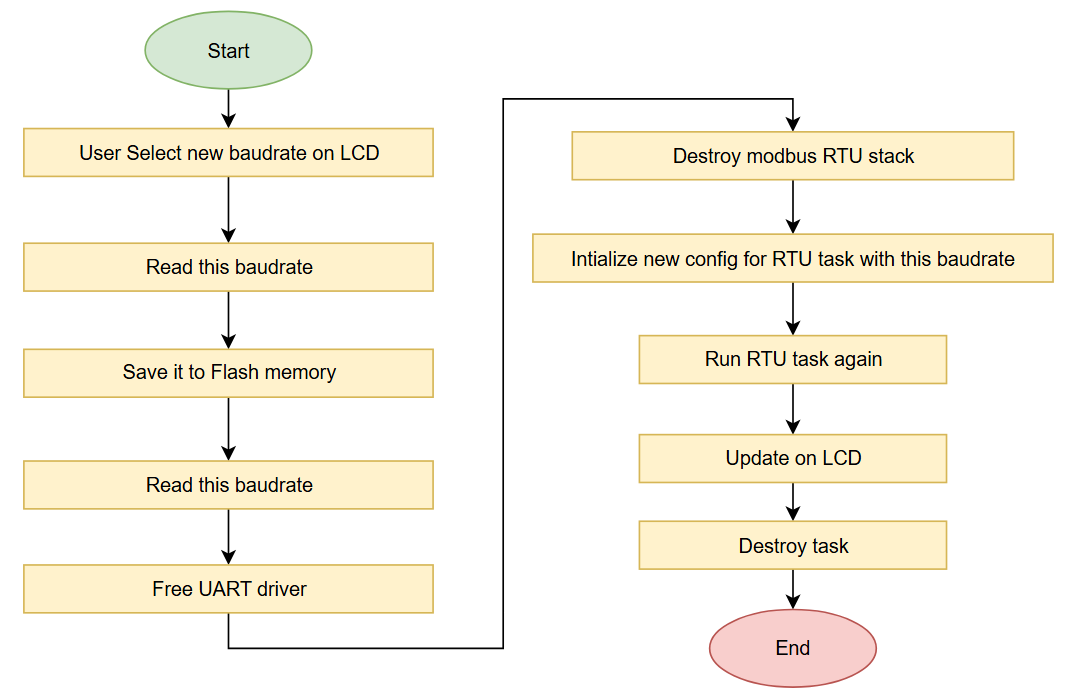
\includegraphics[width=0.85\textwidth]{image/baud_task.png}
    \caption{Lưu đồ giải thuật thực hiện thay đổi tốc độ baudrate}
    \label{fig: baud_task}
\end{figure}
\begin{itemize}
    \item \textbf{User Select new baudrate on LCD: } Người dùng chọn một giá trị tốc độ 
    baud mới thông qua giao diện màn hình LCD.
    \item \textbf{Read this baudrate:} Hệ thống ghi nhận và xử lý giá trị đã chọn từ đầu vào.
    \item \textbf{Save it to Flash memory:} Lưu tốc độ baud mới vào bộ nhớ Flash để đảm bảo 
    thông tin không bị mất khi mất điện hoặc khởi động lại.
    \item \textbf{Read this baudrate:} Hệ thống đọc lại giá trị vừa lưu từ Flash để kiểm tra và xác nhận.
    \item \textbf{Free UART driver:} Giải phóng driver UART hiện tại để nạp cấu hình mới.
    \item \textbf{Destroy modbus RTU stack:} Hủy bỏ ngăn xếp (stack) Modbus RTU cũ để chuẩn bị cho một thiết lập mới.
    \item \textbf{Initialize new config for RTU task with this baudrate:} Khởi tạo cấu hình mới cho tác vụ RTU với tốc độ baud vừa được cập nhật.
    \item \textbf{Run RTU task again:} Khởi chạy lại tác vụ truyền thông Modbus RTU với các thông số cấu hình mới.
    \item \textbf{Update on LCD:} Cập nhật trạng thái hoặc tốc độ baud mới lên màn hình LCD cho người dùng.
    \item \textbf{Destroy task:} Giải phóng task cấu hình tạm thời sau khi hệ thống đã cập nhật thành công.
\end{itemize}

\begin{figure}[H]
    \centering
    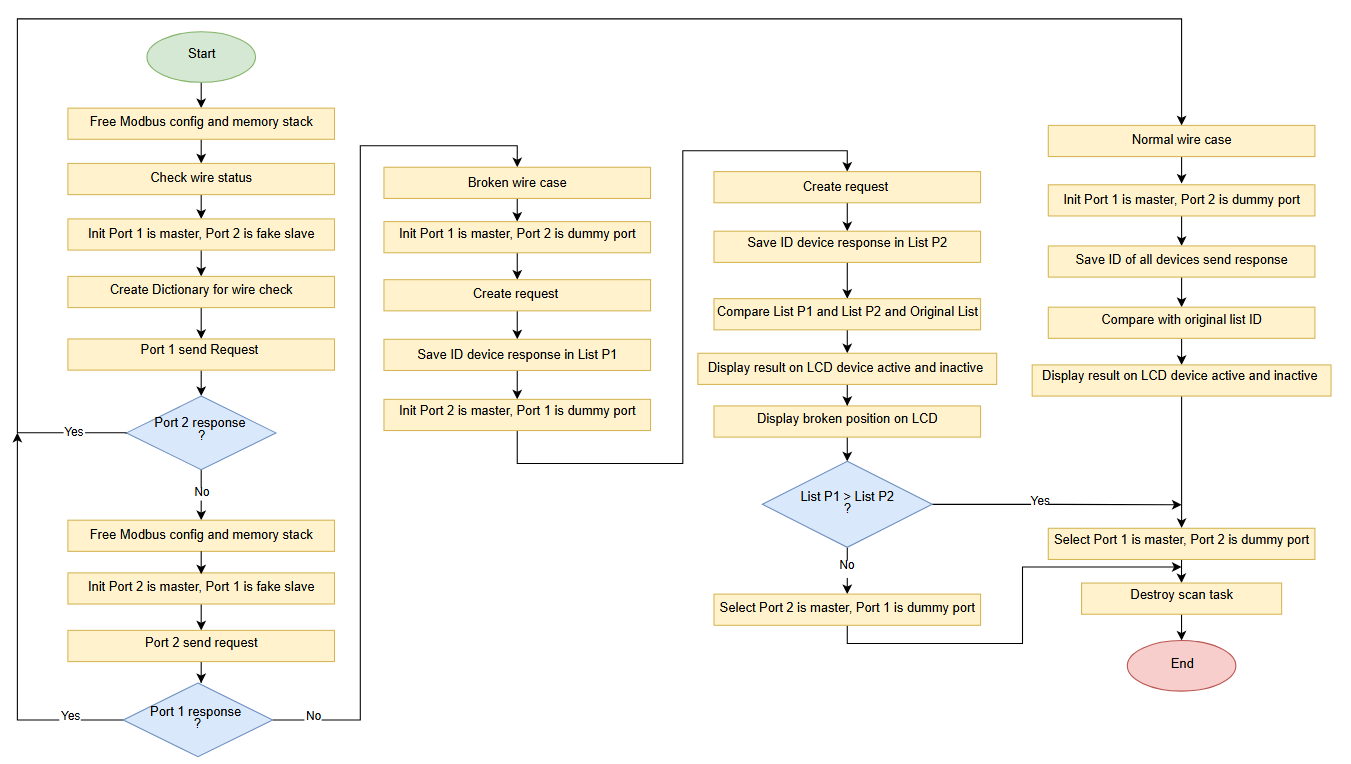
\includegraphics[width=1.1\textwidth]{image/scan_task.png}
    \caption{Lưu đồ giải thuật chức năng scan đường dây}
    \label{fig:scan_task}
\end{figure}
Ý tưởng để thực hiện task scan là thực hiện thay phiên nhau hai port gửi các gói tin ra đường truyền và tách lấy các ID từ các gói tin phản hồi gửi về, ta chia quá trình scan này thành
hai giai đoạn, giai đoạn một sẽ thực hiện gửi các request nhằm xác định đường truyền có đang bị gián đoạn không, giai đoạn hai ta sẽ thực hiện việc tìm chính xác tại điểm gián đoạn đó
ở đoạn nào trên đường truyền, cụ thể như sau:

\textbf{Giai đoạn 1:} thực hiện kiểm tra đường truyền có đứt dây tại đoạn nào không:
\begin{itemize}
    \item Ban đầu sẽ thực xóa các task liên quan tới modbus hiện tại.
    \item cấu hình Port 1 làm Master Port 2 làm Slave, Port 1 tạo các request và đợi Port 2 Slave phần hồi
    \item Nếu Slave 2 phản hồi thì ta kết luận đường truyền không đứt.
    \item Nếu Slave 2 không phản hồi tức là Timeout, ta chuyển sang Port 2 làm Master và Port 1 làm Slave.
    \item Tương tự với trường hợp làm với Port 1, ta cũng chờ Port 1 phản hồi.
    \item Nếu Slave 1 phản hồi thì ta kết luận đường truyền không đứt.
    \item Nếu Slave 1 không phản hồi ta kết luận đường truyền đang gián đoạn.
\end{itemize}

\textbf{Giai đoạn 2:} thực hiện kiểm tra đường truyền gián đoạn tại đâu (nếu có):
\begin{itemize}
    \item cấu hình Port 1 làm Master Port 2 làm Slave, Port 1 tạo các request và đợi các đồng hồ phản hồi.
    \item Ta tiến hành tách lấy phần ID từ những gói tin phản hồi và lưu vào List P1 (Tức là List gồm các ID phản hồi về Port 1)
    \item cấu hình Port 2 làm Master Port 1 làm Slave, Port 2 tạo các request và đợi các đồng hồ phản hồi.
    \item Ta tiến hành tách lấy phần ID từ những gói tin phản hồi và lưu vào List P2 (Tức là List gồm các ID phản hồi về Port 2)
    \item Khi này ta sẽ tiến hành so sánh ID có trong các List với List chứa các ID gốc đang có trong bảng tra của thiết bị.
    \item Nếu cả hai port đều không nhận được response từ một ID tức là tại đó thiết bị đang không hoạt động.
    \item Nếu port 1 chỉ tìm thấy các ID đầu của List chứa ID gốc và port 2 đang chứa các ID ở cuối List gốc, thì ta có thể kết luận vị trí gián đoạn đang ở giữa hai ID cuối của mỗi List.
    \item Nếu so sánh với List ID gốc mà port 1 không nhận được scan nào nhưng port thì có đủ tức là đường truyền đang bị gián đoạn tại đầu port 1 và ngược lại ta kết luận với port 2.
    \item Khi này sau khi đã có được kết quả scan đường truyền thì ta sẽ dựa trên kết quả này để chọn port cho việc thu thập dữ liệu
    \item Nếu đường truyền ổn định thì ta chọn mặc định port 1 làm port thu thập dữ liệu.
    \item Nếu đường truyền gián đoạn thì ta sẽ chọn port có số lượng ID thu thập được lớn hơn làm port thu thập dữ liệu.
    \item Sau cùng ta thực xóa stack của task scan và khôi phục lại task thu thập dữ liệu ban đầu với kết quả port mà ta vừa chọn sau khi scan đường truyền.
\end{itemize}

\begin{figure}[H]
    \centering
    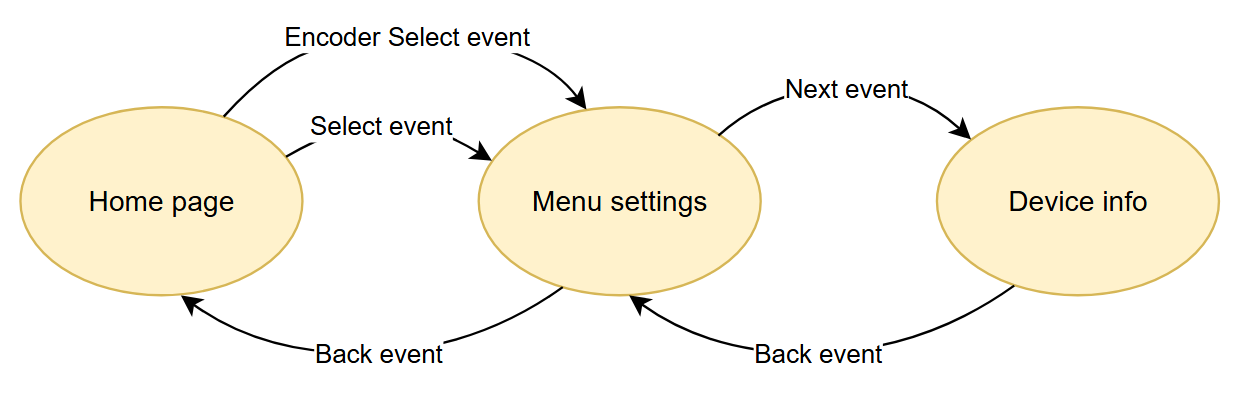
\includegraphics[width=0.8\textwidth]{image/SM_1.png}
    \caption{State machine mô tả chuyển trang của LCD}
    \label{fig:SM_1}
\end{figure}
\begin{figure}[H]
    \centering
    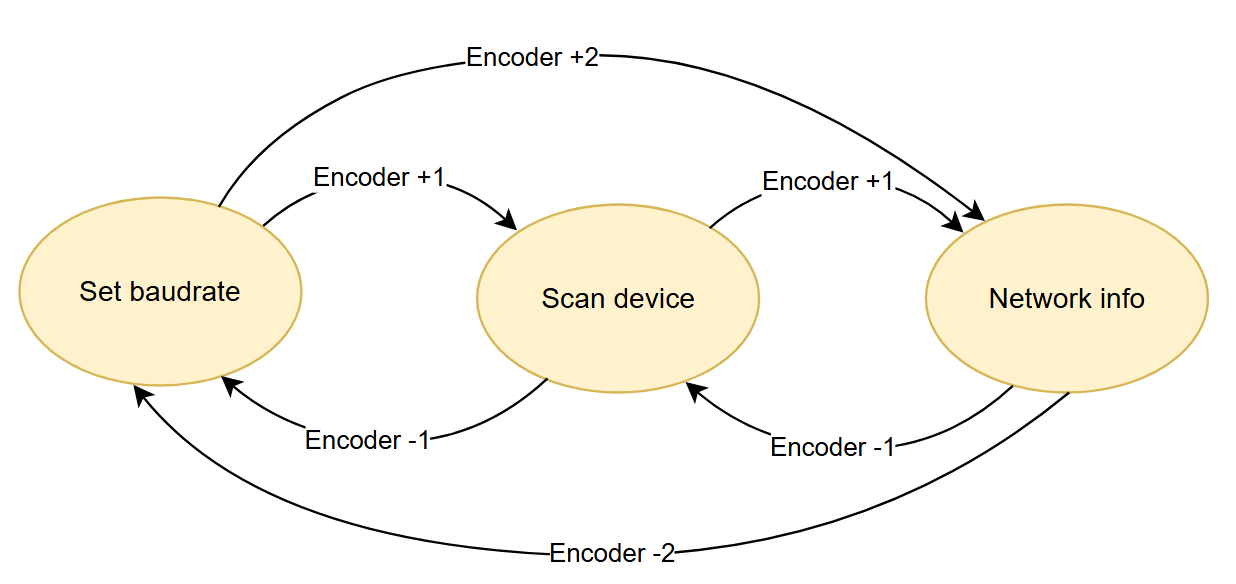
\includegraphics[width=0.8\textwidth]{image/SM_2.png}
    \caption{State machine mô tả trang Menu settings}
    \label{fig:SM_2}
\end{figure}
Màn hình LCD hiển thị ba trang chính, gồm: Home, Menu settings và Device info
Các tín hiệu được sử dụng để điều hướng các trang đến từ các nút nhấn, ví trí quay của encoder và nút nhấn được tích hợp trên encoder thông qua các sự kiện:
\begin{itemize}
    \item \textbf{Select event và Encoder Select event}: đứng tại trang Home và nhận được tín hiệu này sẽ vào trang Menu settings.
    \item \textbf{Next event}: Chuyển qua trang kế tiếp.
    \item \textbf{Back event}: Lùi về một trang trước trang đang đứng
    \item \textbf{Encoder+n}: vị trí xoay tới hiện tại của encoder so với vị trí ban đầu tăng lên n đơn vị.
    \item \textbf{Encoder-n}: vị trí xoay tới hiện tại của encoder so với vị trí ban đầu giảm xuống n đơn vị.
\end{itemize}

Mục Home thể hiện các thông tin trạng thái kết nối với Wi-Fi, Ethernet, Bluetooth và thời gian hiện tại.

Mục Menu settings được sử dụng để hiển thị cho các mục chức năng chính và di chuyển giữa các mục sẽ dựa trên vị trí hiện tại của encoder so với vị trí ban đầu trước khi quay,
mà con trỏ trên màn hình sẽ quyết định di chuyển lên hay di chuyển xuống theo ý người dùng, các chức năng gồm:
\begin{itemize}
    \item \textbf{Set baudrate}: Cài đặt tốc độ baudrate cho thiết bị trong quá trình thu thập dữ liệu từ các đồng hồ điện.
    \item \textbf{Scan device}: Thực hiện chức năng scan đường truyền khi người dùng nhấn chọn vào mục này.
    \item \textbf{Network info}: Sử dụng để xem các thông tin về mạng kết nối của thiết bị.
\end{itemize}

Mục Device info được sử dụng để hiển thị các thông như ID để phục vụ cho việc kết nối và gửi dữ liệu lên Web người dùng và các
thông tin như tên thiết bị, thời gian hoạt động của thiết bị, phiên bản hiện tại của phần mềm và phần cứng của thiết bị.
\begin{figure}[H]
    \centering
    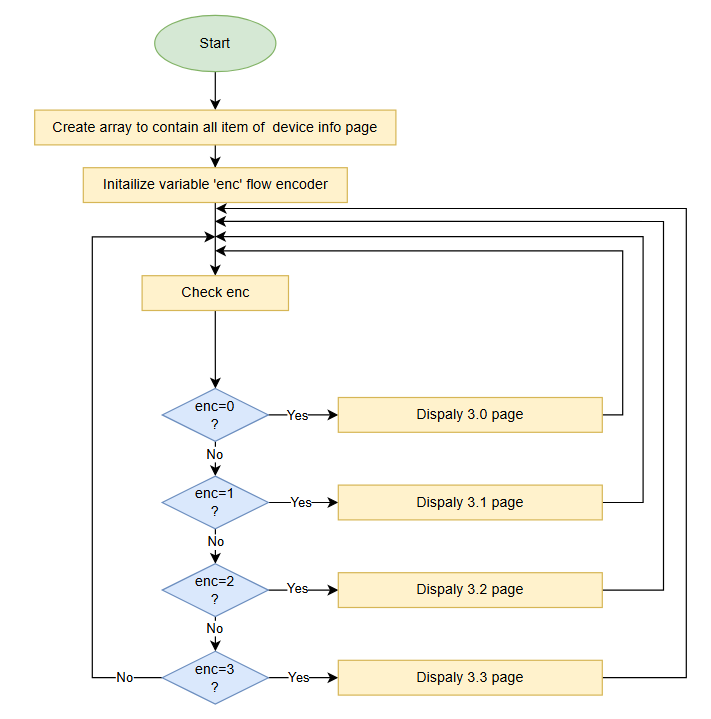
\includegraphics[width=0.8\textwidth]{image/lcd_page_3.png}
    \caption{Lưu đồ giải thuật mô tả hoạt động của trang Device info}
    \label{fig:lcd_page_3}
\end{figure}
Trang này sử dụng với chức năng xem các thông tin của thiết bị.

Ý tưởng sử dụng một biến dùng để đếm số nấc của encoder và di chuyển đến vị trí tiếp theo.

Khi lăn encoder theo chiều kim đồng hồ thì biến đếm sẽ tăng lên và di chuyển xuống các mục phía dưới.

Ngược lại khi lăn ngược chiều kim đồng hồ thì biến đếm sẽ giảm và trở lại các vị trí trang ban đầu.

\section{Thiết kế phần mềm App nhập dữ liệu}
\subsection{Thiết kế phần mềm}
\begin{figure}[H]
    \centering
    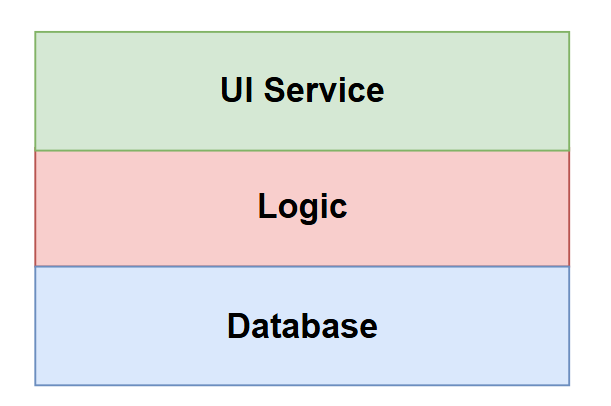
\includegraphics[width=0.4\textwidth]{image/flowchart_tong_quat_2.png}
    \caption{Sơ đồ khối tổng quát của phần mềm App}
    \label{fig:flowchart_tong_quat_2}
\end{figure}
Cấu trúc của giải thuật App gồm có ba phần thực hiện các tác vụ hỗ trợ cho phần còn lại.
Trong đồ án này sử dụng thư viện pyQT sử dụng ngôn ngữ Python, được phát triển lên từ thư viện C++ QT, thư viện này
hỗ trợ cho phép người dùng tạo ra các ô nhập liệu, nút bấm và dựng cửa sổ giao diện bằng cách sử dụng các API đã được
phát triển.
\begin{itemize}
    \item \textbf{UI Service:} render giao diện người dùng bằng thư viện pyQT.
    \item \textbf{Logic:} Sử lý các tác vụ lưu thông tin người dùng nhập, xử lý dữ liệu, gửi dữ liệu xuống thiết bị.
    \item \textbf{Database:} Sử dụng database SQLite để lưu trữ các thông tin mà người dùng nhập và lịch sử nhập liệu và gửi dữ liệu.
\end{itemize}

\begin{figure}[H]
    \centering
    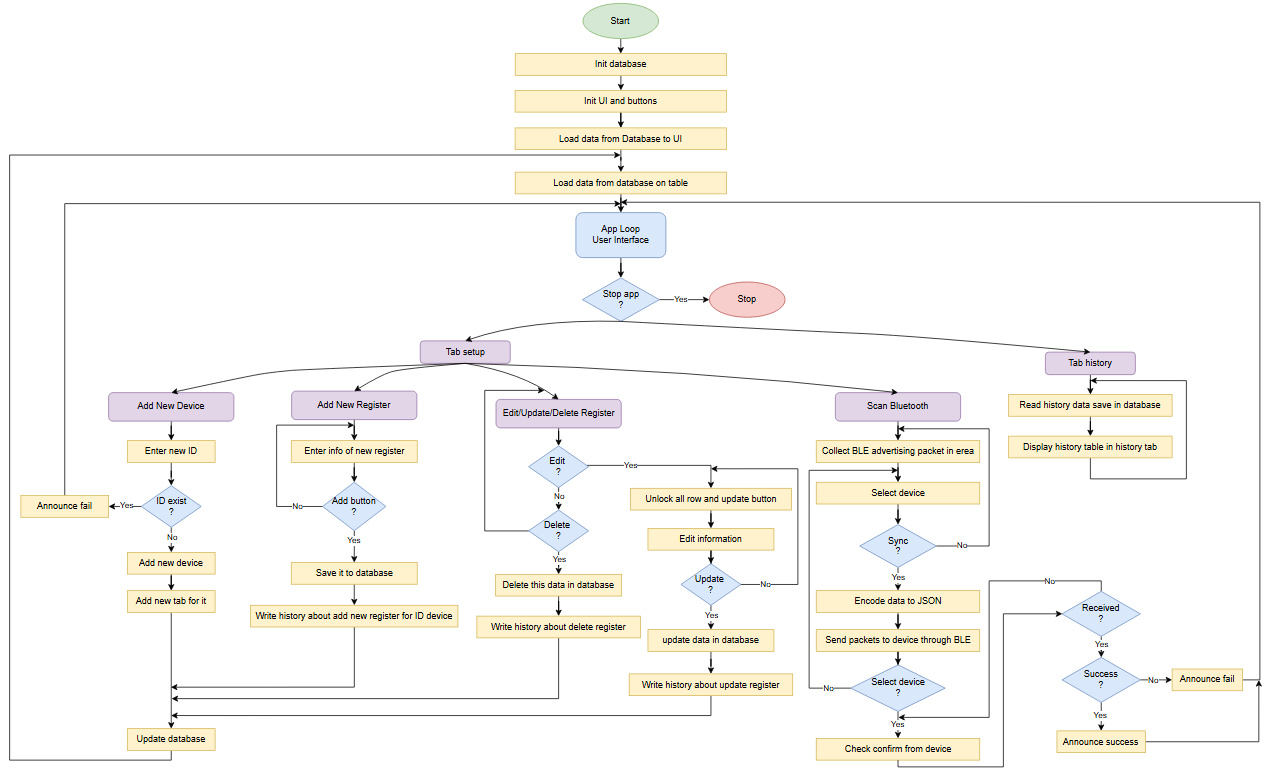
\includegraphics[width=1.1\textwidth]{image/ui_flow.png}
    \caption{Lưu đồ giải thuật chi tiết cho giao diện App }
    \label{fig:ui_flow}
\end{figure}

\begin{figure}[H]
    \centering
    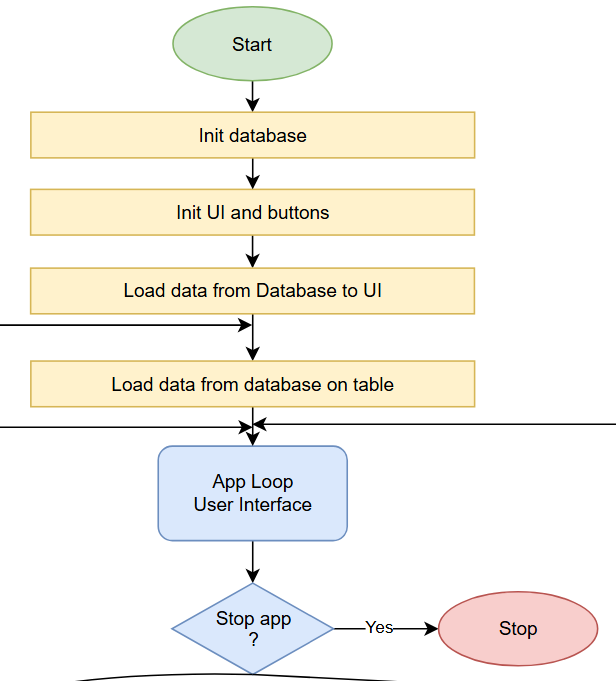
\includegraphics[width=0.5\textwidth]{image/init_ui.png}
    \caption{Lưu đồ giải thuật phần khởi động App}
    \label{fig:init_ui}
\end{figure}
Quá trình này diễn ra khi người dùng bắt đầu mở ứng dụng:
\begin{itemize}
    \item \textbf{Connect signal:} Gắn liên kết nút nhấn với hàm thực hiện chức năng của nút nhấn.
    \item \textbf{Init tab window on UI:} Khởi tạo các khung hình có trên App.
    \item \textbf{Init controller block-Logic:} Khởi tạo các hàm xử lý dữ liệu chính của App.
    \item \textbf{Init Database if not have:} Khởi tạo file để lưu trữ dữ liệu nếu chưa có trong thư mục.
    \item \textbf{Load data from database on table:}: cập nhật các dữ liệu đã định sẵn lên App người dùng có thể thấy được.
    \item \textbf{App Loop User Interface:} bước vào vòng lặp khi người dùng bắt đầu tương tác với App.
    \item \textbf{Stop app:} Kiểm tra có tắt app không.\\
    \textbf{Yes:} Tiến hành đóng App và kết thúc vòng lặp.\\
    \textbf{No:} Tiêp tục quá trình vòng lặp.
\end{itemize}


\begin{figure}[H]
    \centering
    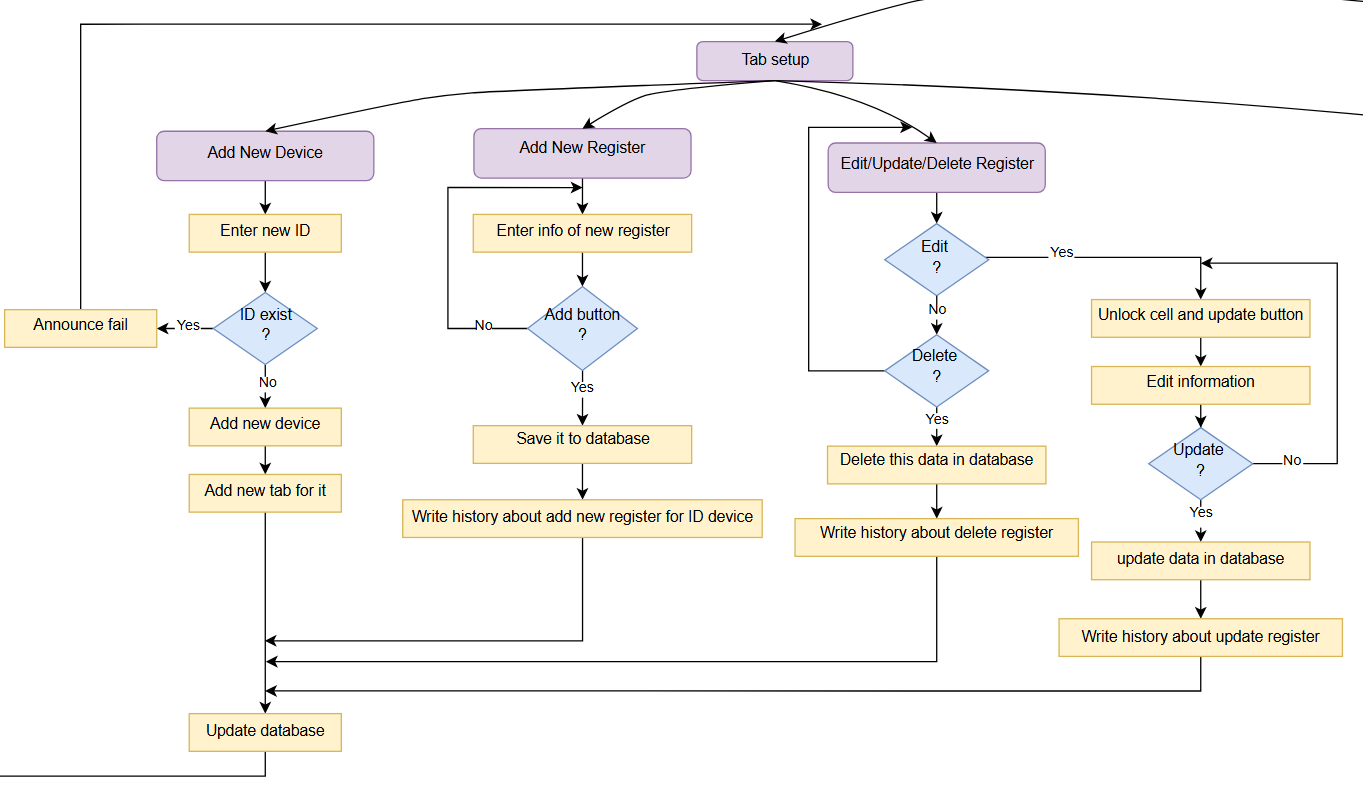
\includegraphics[width=1.1\textwidth]{image/setup_ui.png}
    \caption{Lưu đồ giải thuật phần tab Setup}
    \label{fig:setup_ui}
\end{figure}
Chức năng tạo mới thiết bị:
\begin{itemize}
    \item \textbf{Enter new ID:} Nhập mới một ID của một thiết bị mới vào hệ thống.
    \item \textbf{ID exist?:} Kiểm tra ID đã tồn tại trong hệ thống chưa.\\
    \textbf{Yes:} In ra thông báo lỗi và quay về giao diện của tab setup\\
    \textbf{No - Add new device:} Tạo mới một thiết bị trong hệ thống.
    \item \textbf{Add new tab for it}: tạo cho thiết bị mới này 1 tab riêng trên cửa sổ.
    \item \textbf{Update database:} Cập nhập lại số lượng và danh sách thanh ghi lưu trong database.
\end{itemize}

Chức năng thêm mới thanh ghi:
\begin{itemize}
    \item \textbf{Enter info of new register:} Nhập các số liệu liên quan tới thanh ghi vào các ô.
    \item \textbf{Add button?:} Kiểm tra ID đã bấm nút Add Regiser trên giao diện chưa.\\
    \textbf{No:} Quay về tiếp tục nhập.\\
    \textbf{Yes:} Tiến hành lưu các thông tin trong ô nhập liệu.
    \item \textbf{Save it to database:} Cập nhập lại số lượng và danh sách thanh ghi lưu trong database.
    \item \textbf{Write history about add new register for ID device}: tiến hành tạo dòng log ở tab history về việc vừa thêm một thanh ghi vào hệ thống.
\end{itemize}

Các chức năng phụ kèm theo Edit/Update/Delete:

Chức năng nút Edit:
\begin{itemize}
    \item \textbf{Edit?:} Kiểm tra nút nhấn Edit có được nhấn không.\\
    \textbf{Yes:} 
    \item \textbf{Unlock cell and update button:} Mở khóa các ô trong bảng và cho phép người dùng thay đổi thông tin.
    \item \textbf{Edit infomation:} Người dùng chỉnh sửa thông tin.
    \textbf{No:} Kiểm tra tiếp nút nhấn Delete.
\end{itemize}

Chức năng nút Delete:
\begin{itemize}
    \item \textbf{Delete?:} Kiểm tra nút nhấn Delete có được nhấn không.\\
    \textbf{No:} tiếp tục chỉnh sửa thông tin trong bảng.\\
    \textbf{Yes:} 
    \item \textbf{Delete this data in database:} Xóa dòng người dùng vừa chọn trong database
    \item \textbf{Write history about delete register}: tiến hành tạo dòng log ở tab history về việc vừa xóa một thanh ghi.
\end{itemize}

Chức năng nút Update:
\begin{itemize}
    \item \textbf{Update?:} Kiểm tra nút nhấn Update có được nhấn không.\\
    \textbf{No:} tiếp tục chỉnh sửa thông tin trong bảng.\\
    \textbf{Yes:} 
    \item \textbf{Update data in database:} Cập nhập lại các thông tin vừa chỉnh sửa vào database.
    \item \textbf{Write history about update register}: tiến hành tạo dòng log ở tab history về việc vừa chỉnh sửa thông tin trong bảng.
\end{itemize}

\begin{figure}[H]
    \centering
    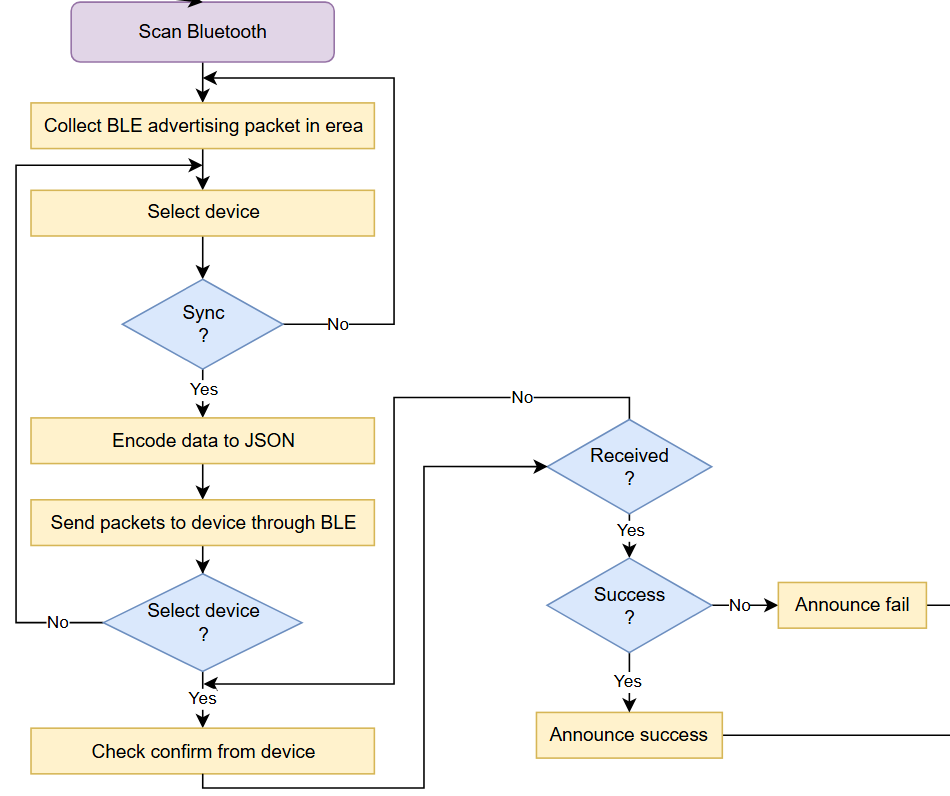
\includegraphics[width=0.8\textwidth]{image/ble_ui.png}
    \caption{Lưu đồ giải thuật phần chức năng Sync}
    \label{fig:ble_ui}
\end{figure}
Chức năng này giúp đóng gói dữ liệu gồm các thanh ghi mà người dùng nhập từ máy tính và gửi xuống cho thiết bị thực hiện thu thập dữ liệu
từ các thanh ghi và các thông số đã nhập trên App:
\begin{itemize}
    \item \textbf{Collect BLE advertising packet in erea:} tìm các thiết bị xung quanh hiện đang phát tín hiệu Bluetooth trong không gian.
    \item \textbf{Select device:} Chọn thiết bị mong muốn gửi dữ liệu.
    \item \textbf{Sync?:} Kiểm tra nút gửi dữ liệu đã được nhấn chưa.\\
    \textbf{No:} Nếu chưa thì tiếp tục tìm các thiết bị và chọn thiết bị.\\
    \textbf{Yes:} nếu đã nhấn nút sync.
    \item \textbf{Encode data to JSON:} Đóng gói toàn bộ dữ liệu thanh ghi theo dạng JSON.
    \item \textbf{Send packets to device through BLE:} chia nhỏ gói tin ra và gửi lần lượt xuống thiết 
    \item \textbf{Select device?:} Kiểm tra đã chọn thiết bị muốn gửi dữ liệu chưa.\\
    \textbf{No:} Thông báo lỗi và yêu cầu chọn thiết bị trước khi gửi.\\
    \textbf(Yes:) Tiến hành gửi dữ liệu và đợi xác nhận từ thiết bị.
    \item \textbf{Received?:} Đợi nhận gói tin phản hồi, nếu chưa có tiếp tục chờ.
    \item \textbf{Success?:} Kiểm tra phản hồi là thành công hay thất bại.\\
    \textbf{No:} In thông báo lỗi ra màn hình.\\
    \textbf{Yes:} Thông báo đã gửi thành công cho thiết bị.
\end{itemize}
\begin{figure}[H]
    \centering
    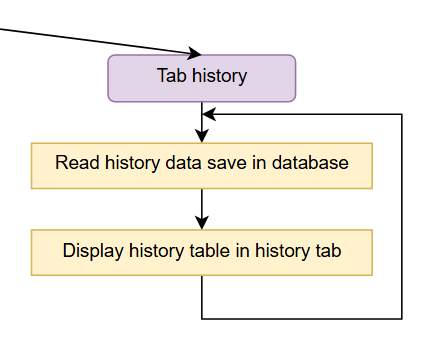
\includegraphics[width=0.4\textwidth]{image/his_tab.png}
    \caption{Lưu đồ giải thuật phần tab History}
    \label{fig:his_tab}
\end{figure}
Sử dụng chủ yếu để hiển thị lịch sử nhập liệu:
\begin{itemize} 
    \item \textbf{Read history date save in database:} Đọc các log đã lưu từ những chức năng khác thêm vào.
    \item \textbf{Display history table in history tab:} Hiển thị các nội dung log vừa đọc dưới dạng bảng ở tab history.
\end{itemize}

\section{Phát triển giao diện Dashboard theo dõi dữ liệu}
\subsection{Thiết kế phần mềm}
\begin{figure}[H]
    \centering
    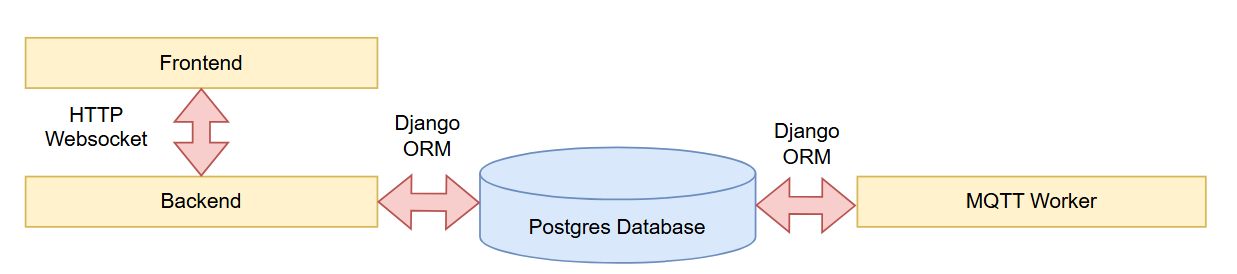
\includegraphics[width=1.1\textwidth]{image/web_flow.png}
    \caption{Sơ đồ tổng quát các phần của trang web}
    \label{fig:web_flow}
\end{figure}
Trang web được phát triển dựa trên một Repo đã có sẵn, chạy trên localhost, trang web này dùng để cập nhật dữ liệu theo thời gian thực 
lên giao diện người dùng thông qua Websocket hoặc HTTP, sử dụng database Postges làm nơi lưu trữ thông tin, giao diện người
dùng được xây dựng dựa trên thư viện React, phần backend sử dụng framework Django.

Trong đồ án này ta xây dựng thêm một tiến trình chạy ngầm song song với backend để thu thập dữ liệu được gửi lên từ thiết thông qua MQTT.
Tiến trình này sẽ thực hiện các công việc cụ thể như đợi gói tin, phân tích gói tin, lưu dữ liệu sau khi đóng gói vào database của trang web.
Với mục đích là hiển thị các thông tin thật lên trang web cho người dùng nhìn trực quan hơn về dữ liệu mà người dùng thu thập được thay vì phải mở terminal hay chỉ xem được tại thiết bị.
\begin{figure}[H]
    \centering
    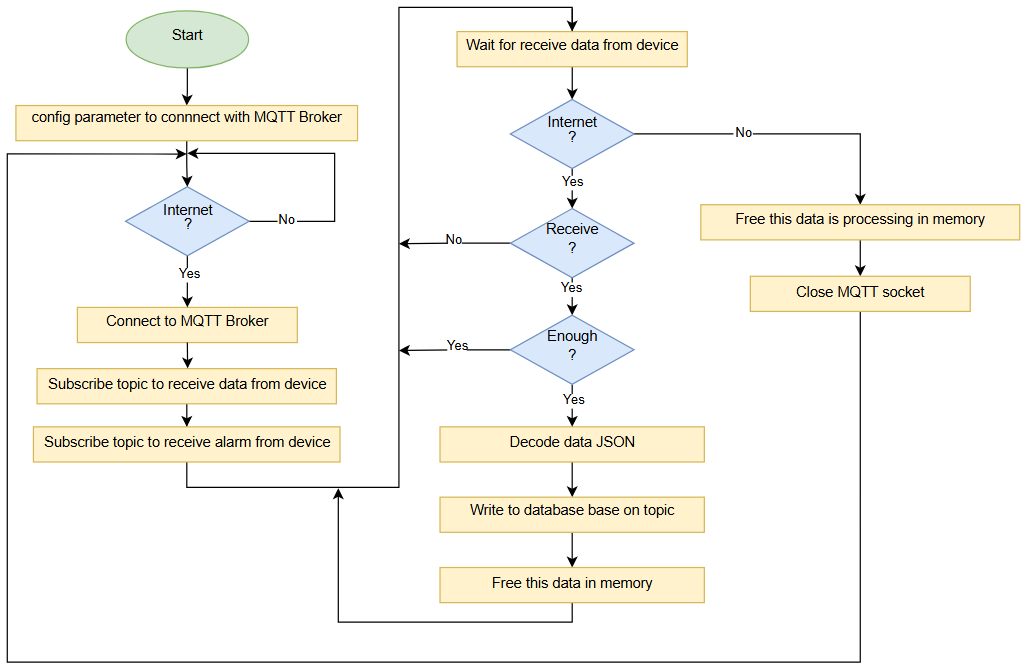
\includegraphics[width=1.1\textwidth]{image/mqtt_web.png}
    \caption{Lưu đồ giải thuật phần nhận dữ liệu từ thiết bị - MQTT Worker}
    \label{fig:mqtt_web}
\end{figure}
Chức năng chính là đăng ký vào các Topic mà thiết bị đã tạo và đợi nhận dữ liệu được gửi từ thiết bị lên MQTT Broker.
 
\begin{itemize}
    \item \textbf{Config parameter to connect with MQTT Broker:} Khởi tạo các thông số liên quan đến giao tiếp MQTT như địa chỉ của broker, cổng kết nối.
    \item \textbf{Internet?:} Kiểm tra tình trạng kết nối mạng của máy chủ.\\
    \textbf{No:} Tiếp tục chờ tới khi có mạng.\\
    \textbf{Yes:} Bắt đầu quá trình nhận dữ liệu từ thiết bị.
    \item \textbf{Connect to MQTT Broker:} Thực hiện kết nối với MQTT broker đã được định nghĩa trước.
    \item \textbf{Subcribe topic to receive data from device:} Đăng ký vào topic nhận dữ liệu đồng hồ điện.
    \item \textbf{Subcribe topic to receive alarm from device:} Đăng ký vào topic nhận cảnh báo khi phát hiện đường truyền lỗi.
    \item \textbf{Wait for receive data from device:} đợi các gói tin thông qua các Topic đã đăng ký với MQTT broker.
    \item \textbf{Internet?:} Kiểm tra tình trạng kết nối mạng hiện tại.\\
    \textbf{No:} Mất kết nối mạng
    \item \textbf{Free this data is proccessing in memory:} Giải phóng vùng nhớ chứa các nội dung đang xử lý của MQTT.
    \item \textbf{Close MQTT socket:} Tắt socket hiện tại tại cổng 1883.\\
    \textbf{Yes:} Nếu có kết nối mạng.
    \item \textbf{Receice?:} Kiểm tra đã bắt được dữ liệu từ MQTT broker không.\\
    \textbf{No:} Tiếp tục quay lại đợi nhận gói tin.\\
    \textbf{Yes:} Kiểm tra tình trạng gói tin.
    \item \textbf{Enough?:} Kiểm tra tình trạng dữ liệu từ message đã đủ chưa.\\
    \textbf{No:} Tiếp tục nhận các gói tin khác.\\
    \textbf{Yes:} Bắt đầu phân tích gói tin.
    \item \textbf{Decode data JSON:} giải mã gói tin JSON.
    \item \textbf{Write to database base on topic:} Tiến hành lưu dữ liệu vào đúng database của web dựa trên topic và thông tin định danh của thiết bị gửi lên.
    \item \textbf{Free this data in memory:} Sau khi đã lưu dữ liệu vào database thì tiến hành dọn dẹp vùng nhớ cũ và tiếp tục kiểm tra và đợi nhận gói tin tiếp theo.
\end{itemize}